\documentclass[10pt,letterpaper]{article}
\usepackage[margin=1in]{geometry}
\usepackage{amsmath,amssymb}
\usepackage{graphicx,booktabs,multirow,longtable,array}
\usepackage{float}
\usepackage{tikz}
\usepackage{pgfplots}\pgfplotsset{compat=1.16}
\usepackage[colorlinks=true,linkcolor=blue,citecolor=blue,urlcolor=blue]{hyperref}
\usepackage{caption}
\captionsetup{font=small,labelfont=bf,skip=6pt}
\usepackage{enumitem}
\setlist{topsep=3pt,itemsep=2pt}
\usepackage{titlesec}
\titlespacing*{\section}{0pt}{12pt plus 2pt}{6pt}
\titlespacing*{\subsection}{0pt}{10pt plus 2pt}{4pt}
\setlength{\parskip}{3pt}
\setlength{\parindent}{0pt}

% --- Bright figure colours ---
\definecolor{myorange}{RGB}{230,126,34}
\definecolor{myblue}{RGB}{41,128,185}
\definecolor{mygreen}{RGB}{39,174,96}
\definecolor{myred}{RGB}{231,76,60}
\definecolor{myblack}{RGB}{44,62,80}
\pgfplotsset{
  every axis/.append style={
    axis background/.style={fill=white},
    grid style={gray!20},
    major grid style={gray!25},
    minor grid style={gray!12},
    tick label style={font=\small},
    label style={font=\small},
    line width=0.7pt,
  },
  every axis plot/.append style={line width=1.2pt, mark size=2.5pt, mark options={solid, fill=white, line width=1pt}}
}

\title{COMPARATIVE ERROR AND CONVERGENCE ANALYSIS OF\\ EXPLICIT SINGLE-STEP NUMERICAL METHODS FOR\\ FIRST-ORDER ORDINARY DIFFERENTIAL EQUATIONS}
\author{SADIQ HARUNA SHEHU$^{1*}$\\[4pt]
\small $^{1}$Department of Mathematics, Faculty of Science,\\ Northwest University, Kano, Nigeria.\\[2pt]
\small Email: sadiqharunashehu016@gmail.com (S. H. Shehu)}
\date{}
\begin{document}
\maketitle

\begin{abstract}
Many first-order initial value problems (IVPs) lack closed-form solutions, so numerical methods are indispensable. This paper compares four explicit single-step methods---Euler, the Modified Euler (Heun) method, the second-order Taylor series method, and the classical fourth-order Runge--Kutta method (RK4)---on seven IVPs over $[0,1]$ (five linear and two nonlinear) with step sizes $h=0.2,\,0.1,\,0.05,\,0.025,\,0.0125$. For the second-order methods, we compute the leading local truncation error (LTE) coefficient of each method and propagate it through the variational equation to obtain an asymptotic global-error constant. These constants predict the observed Heun-versus-Taylor error ratios on all seven problems (for example, a predicted ratio of $7.00$ against an observed $6.71$ for $y'=ty$ at $h=0.0125$). For constant-coefficient linear ODEs, Heun and Taylor are shown to be algebraically identical. Least-squares convergence orders over all five step sizes were $0.95$--$1.06$ (Euler), $1.95$--$2.11$ (Heun), $1.93$--$2.03$ (Taylor) and $3.95$--$4.14$ (RK4). RK4 was the most accurate on every problem, with maximum errors between $9\times10^{-7}$ and $6\times10^{-5}$ at $h=0.2$. For one test problem and a fixed target error, RK4 needed about $2{,}200$ times fewer function evaluations than Euler and about $12$ times fewer than Heun. The conclusions apply to the non-stiff problems tested here.
\end{abstract}

\noindent\textbf{Keywords :} numerical methods, ordinary differential equations, error analysis, convergence order, local truncation error, Runge--Kutta methods.

\section{Introduction}
Ordinary differential equations (ODEs) describe how quantities change with an independent variable and appear throughout physics, engineering and applied mathematics [1,2]. A first-order initial value problem (IVP) is written
\begin{equation}
\frac{dy}{dt}=f(t,y),\qquad y(t_0)=y_0. \label{eq:ivp}
\end{equation}
Some first-order ODEs can be solved exactly by separation of variables or integrating factors, but many practical equations cannot, and numerical approximation is then the only route.

Standard texts [3,4,5,6,7] present Euler's method, the Modified Euler method, Taylor series methods and the Runge--Kutta family, which differ in order, stability and cost [8]. Several studies compare these methods empirically on test problems [9,10,11,12]. Such comparisons usually report error magnitudes or global convergence rates. The asymptotic theory that links the local truncation error to the global error is classical [14,2], but it is rarely worked through side by side for several second-order methods on concrete test problems.

This paper provides such a worked comparison. We (1) quantify the accuracy of the four methods on seven test problems, including two nonlinear ones; (2) check the theoretical convergence orders empirically; and (3) use the leading LTE coefficients, propagated to global-error constants, to explain which second-order method wins on which problem, and why Heun and Taylor coincide for constant-coefficient linear ODEs. The LTE argument is a predictive heuristic grounded in the asymptotic error expansion, not a new theorem, and we test it against the computed errors rather than assume it.

\section{Mathematical Formulation}
We consider the IVP $y'=f(t,y)$, $y(t_0)=y_0$, $t\in[t_0,t_f]$, on $[0,1]$. With the uniform grid $t_n=t_0+nh$, $h=(t_f-t_0)/N$, the numerical approximation to $y(t_n)$ is $y_n$. The seven test problems, each with a known exact solution used as the benchmark, are:
\begin{enumerate}
\item \textbf{Affine, constant coefficients:} $y'=t+y$, $y(0)=1$; $y=2e^{t}-t-1$.
\item \textbf{Linear homogeneous, variable coefficient (separable):} $y'=ty$, $y(0)=1$; $y=e^{t^2/2}$.
\item \textbf{Linear, polynomial forcing:} $y'=y-t^2+1$, $y(0)=0.5$; $y=t^2+2t+1-0.5e^{t}$.
\item \textbf{Linear, trigonometric forcing:} $y'=\cos t-y$, $y(0)=0$; $y=\tfrac12(\sin t+\cos t-e^{-t})$.
\item \textbf{Applied (Newton's law of cooling):} $T'=-0.5(T-25)$, $T(0)=100$; $T=25+75e^{-0.5t}$. This is again an affine, constant-coefficient problem and so belongs to the same class as Problem~1.
\item \textbf{Nonlinear (logistic):} $y'=y(1-y)$, $y(0)=0.1$; $y=1/(1+9e^{-t})$.
\item \textbf{Nonlinear, separable:} $y'=-2ty^2$, $y(0)=1$; $y=1/(1+t^2)$.
\end{enumerate}
Problems 1--5 are all linear in $y$; they differ in whether the coefficients are constant and in the form of the forcing term. Problems 6 and 7 were added so that the conclusions are not restricted to linear equations.

\section{Numerical Methods}
``Modified Euler'' denotes Heun's predictor--corrector scheme. The five step sizes used are 0.2, 0.1, 0.05, 0.025 and 0.0125. The methods are:
\begin{align}
\text{Euler:}\quad & y_{n+1}=y_n+hf(t_n,y_n),\\
\text{Heun:}\quad & \tilde y_{n+1}=y_n+hf(t_n,y_n),\notag\\
& y_{n+1}=y_n+\tfrac h2\big[f(t_n,y_n)+f(t_{n+1},\tilde y_{n+1})\big],\label{eq:heun}\\
\text{Taylor-2 ($Df=f_t+ff_y$):}\quad & y_{n+1}=y_n+hf(t_n,y_n)+\tfrac{h^2}{2}Df(t_n,y_n),\label{eq:taylor}
\end{align}
and the classical RK4 scheme [13]:
\begin{align}
k_1&=f(t_n,y_n), & k_2&=f(t_n+\tfrac h2,y_n+\tfrac h2k_1),\\
k_3&=f(t_n+\tfrac h2,y_n+\tfrac h2k_2), & k_4&=f(t_n+h,y_n+hk_3),\\
y_{n+1}&=y_n+\tfrac h6(k_1+2k_2+2k_3+k_4).
\end{align}
Table~1 lists the total derivatives $Df$ needed by the Taylor method.

\begin{table}[H]\centering
\caption{Total derivatives $Df=f_t+ff_y$ for the Taylor method.}
\begin{tabular}{@{}clc@{}}\toprule
Problem & $f(t,y)$ & $Df(t,y)$\\\midrule
1 & $t+y$ & $1+t+y$\\
2 & $ty$ & $y+t^2y$\\
3 & $y-t^2+1$ & $-2t+y-t^2+1$\\
4 & $\cos t-y$ & $-\sin t-\cos t+y$\\
5 & $-0.5(T-25)$ & $0.25(T-25)$\\
6 & $y(1-y)$ & $(1-2y)\,y(1-y)$\\
7 & $-2ty^2$ & $-2y^2+8t^2y^3$\\\bottomrule
\end{tabular}
\end{table}

\section{Error Analysis, Consistency and Convergence}
Let $E_n=y(t_n)-y_n$ be the global error and $E_{\max}=\max_n|E_n|$. For a one-step method $y_{n+1}=y_n+h\Phi(t_n,y_n,h)$, the local truncation error (the local defect, not divided by $h$) is
\begin{equation}
\tau_{n+1}=y(t_{n+1})-y(t_n)-h\Phi(t_n,y(t_n),h).\label{eq:lte}
\end{equation}
For a method of order $p$, $\tau_{n+1}=O(h^{p+1})$. The method is consistent if $\Phi(t,y,0)=f(t,y)$. If $f$ is Lipschitz in $y$, consistency implies convergence of a one-step method, and $E_n=O(h^{p})$.

\paragraph{Empirical order.} We report two estimates. The \emph{pairwise} order from the two finest step sizes is
\begin{equation}
\hat p=\log_2\!\big(E_{\max}(0.025)/E_{\max}(0.0125)\big),
\end{equation}
which follows from $E(h)\approx Ch^p$. The \emph{fitted} order is the least-squares slope of $\log E_{\max}$ against $\log h$ over all five step sizes. Both are estimates; pre-asymptotic behaviour at large $h$ can shift them slightly from the integer values.

\paragraph{Verification.} All computations were carried out in MATLAB. The full set of results (all seven problems, all four methods, all five step sizes) was independently recomputed in a second implementation, and the maximum errors agreed with the MATLAB values to the four significant figures reported in Table~3. Hand calculation of the first three steps of Problem~1 also matched. Code is available at \url{https://github.com/Sadiq-Dambatta/single-step-ODE-methods}.

\section{Analytical Comparison of the Second-Order Methods}
\subsection{Leading LTE terms and global-error constants}
Along the exact solution, the leading ($O(h^3)$) LTE terms are
\begin{align}
\tau_{\text{Taylor}}&=\frac{h^3}{6}\,y'''(t)+O(h^4),\label{eq:tt}\\
\tau_{\text{Heun}}&=\frac{h^3}{12}\Big[-(f_{tt}+2ff_{ty}+f^2f_{yy})+2f_y(f_t+ff_y)\Big]+O(h^4).\label{eq:th}
\end{align}
Write $\tau=h^3c(t)$ for the leading term. A pointwise comparison of $|c(t)|$ is only a local statement, because the global error accumulates the defects introduced at all earlier steps. By the asymptotic expansion of the global error for one-step methods [14,2], $E(t)=h^2e(t)+O(h^3)$ where $e$ solves the variational equation
\begin{equation}
e'(t)=f_y\big(t,y(t)\big)\,e(t)+c(t),\qquad e(0)=0.\label{eq:var}
\end{equation}
We therefore define the \emph{asymptotic global-error constant} $C=\max_{t\in[0,1]}|e(t)|$ for each method and compare these constants. They are computed by solving \eqref{eq:var} numerically with $c(t)$ evaluated symbolically on the exact solution.

\subsection{Case 1: constant-coefficient linear ODEs (Problems 1 and 5)}
Let $f=at+by+c_0$. Then $f_{tt}=f_{ty}=f_{yy}=0$ and $Df=a+bf$, so
\[
f\big(t+h,\,y+hf\big)=a(t+h)+b(y+hf)+c_0=f+h(a+bf)=f+h\,Df\quad\text{exactly}.
\]
Substituting into \eqref{eq:heun} gives $y_{n+1}=y_n+\tfrac h2\big[2f+h\,Df\big]=y_n+hf+\tfrac{h^2}{2}Df$, which is \eqref{eq:taylor}. Heun and Taylor-2 are therefore algebraically identical for these problems, and the errors in Table~3 coincide to every digit reported.

\subsection{Case 2: $y'=ty$ (Problem 2)}
Here $f_t=y$, $f_y=t$, $f_{tt}=0$, $f_{ty}=1$, $f_{yy}=0$ and $y=e^{t^2/2}$. Then
\begin{equation}
c_{\text{Heun}}=\frac{t^3y}{6},\qquad c_{\text{Taylor}}=\frac{y'''}{6}=\frac{ty(t^2+3)}{6}.
\end{equation}
The pointwise ratio $c_{\text{Taylor}}/c_{\text{Heun}}=(t^2+3)/t^2$ equals $76$ at $t=0.2$ but only $4$ at $t=1$, and it is unbounded as $t\to0$; it is therefore not a reliable predictor of the global errors. Solving \eqref{eq:var} in closed form with $f_y=t$ gives $e(t)=e^{t^2/2}\int_0^t e^{-s^2/2}c(s)\,ds$, and since $c(s)\propto e^{s^2/2}$,
\begin{align}
e_{\text{Heun}}(1)&=\frac{e^{1/2}}{6}\int_0^1 s^3\,ds=\frac{e^{1/2}}{24}\approx0.0687,\\
e_{\text{Taylor}}(1)&=\frac{e^{1/2}}{6}\int_0^1 (s^3+3s)\,ds=\frac{7e^{1/2}}{24}\approx0.4809.
\end{align}
The predicted error ratio is exactly $7$. The observed ratio of maximum errors rises towards this value as $h$ decreases ($5.9$ at $h=0.05$, $6.7$ at $h=0.0125$). The prediction also matches the magnitudes: $h^2e_{\text{Taylor}}(1)=7.5\times10^{-5}$ at $h=0.0125$, against $7.41\times10^{-5}$ observed.

\subsection{Case 3: $y'=y-t^2+1$ (Problem 3)}
With $f_t=-2t$, $f_y=1$, $f_{tt}=-2$ and $f_{ty}=f_{yy}=0$,
\begin{equation}
c_{\text{Heun}}=\frac16\big[y-t^2-2t+2\big]=\frac16\big(3-0.5e^{t}\big),\qquad c_{\text{Taylor}}=\frac{y'''}{6}=-\frac{0.5e^{t}}{6}.
\end{equation}
For all $t\in[0,1]$, $0.5e^{t}\le1.359<1.641\le3-0.5e^{t}$, so $|c_{\text{Taylor}}|<|c_{\text{Heun}}|$ pointwise. The accumulated constants in Table~2 agree: Taylor is about $0.36$ times as large as Heun, as observed.

\subsection{Case 4: $y'=\cos t-y$ (Problem 4)}
Here $f_t=-\sin t$, $f_y=-1$, $f_{tt}=-\cos t$ and $f_{ty}=f_{yy}=0$. On the exact solution,
\begin{equation}
c_{\text{Heun}}=\frac{1}{12}\big(2\cos t+\sin t+e^{-t}\big),\qquad c_{\text{Taylor}}=\frac{1}{12}\big(\sin t-\cos t+e^{-t}\big).
\end{equation}
At $t=0$ the Taylor coefficient vanishes while Heun's equals $1/4$, and Taylor's remains much smaller on $[0,1]$. This explains why Taylor is about ten times more accurate than Heun on this problem (Table~2).

\subsection{Nonlinear problems (Problems 6 and 7)}
For the nonlinear problems the same symbolic procedure applies, with $c(t)$ and $f_y$ evaluated on the exact solution. Table~2 shows that the predicted ratio again matches the observed one: Taylor is better than Heun on the logistic problem (ratio $0.35$), and worse on Problem~7 (ratio $2.5$). In Problem~7 the Taylor coefficient $c_{\text{Taylor}}$ vanishes at $t=1$ but is large for $t\approx0.2$--$0.5$, and the accumulated constant, not the endpoint value, determines the outcome.

\begin{table}[H]\centering
\caption{Predicted asymptotic global-error constants $C$ (maximum of $|e(t)|$ from \eqref{eq:var}) and the predicted and observed Taylor/Heun error ratios. The observed ratio uses $E_{\max}$ at $h=0.0125$.}
\begin{tabular}{@{}ccccc@{}}\toprule
Problem & $C_{\text{Heun}}$ & $C_{\text{Taylor}}$ & \multicolumn{2}{c}{Ratio Taylor/Heun} \\
\cmidrule(lr){4-5}
 & & & Predicted & Observed\\\midrule
1 & 0.9061 & 0.9061 & 1.00 & 1.00 \\
2 & 0.0687 & 0.4809 & 7.00 & 6.71 \\
3 & 0.6326 & 0.2265 & 0.36 & 0.36 \\
4 & 0.1430 & 0.0163 & 0.11 & 0.11 \\
5 & 0.9477 & 0.9477 & 1.00 & 1.00 \\
6 & 0.0179 & 0.0062 & 0.35 & 0.35 \\
7 & 0.0966 & 0.2401 & 2.49 & 2.51\\
\bottomrule\end{tabular}
\end{table}

\section{Numerical Results and Discussion}
\subsection{Accuracy}
Table~3 gives the maximum absolute errors. RK4 is the most accurate on all seven problems and all step sizes, with errors between $9.2\times10^{-7}$ and $6.1\times10^{-5}$ at $h=0.2$, falling to between $1.6\times10^{-11}$ and $1.1\times10^{-9}$ at $h=0.0125$. Euler is the least accurate throughout. Among the second-order methods, the winner depends on the problem, as predicted in Section~5: they tie on Problems 1 and 5, Heun wins on Problems 2 and 7, and Taylor wins on Problems 3, 4 and 6.

{\footnotesize
\begin{longtable}{@{}llcccc@{}}
\caption{Maximum absolute errors $E_{\max}$ for all problems and step sizes.}\\
\toprule
Problem & $h$ & Euler & Mod.\ Euler & Taylor-2 & RK4\\\midrule
\endfirsthead
\toprule Problem & $h$ & Euler & Mod.\ Euler & Taylor-2 & RK4\\\midrule
\endhead
\multirow{5}{*}{1 (Affine)} & 0.2 & $4.599\times10^{-1}$ & $3.115\times10^{-2}$ & $3.115\times10^{-2}$ & $6.138\times10^{-5}$ \\
 & 0.1 & $2.491\times10^{-1}$ & $8.402\times10^{-3}$ & $8.402\times10^{-3}$ & $4.169\times10^{-6}$ \\
 & 0.05 & $1.300\times10^{-1}$ & $2.182\times10^{-3}$ & $2.182\times10^{-3}$ & $2.716\times10^{-7}$ \\
 & 0.025 & $6.644\times10^{-2}$ & $5.558\times10^{-4}$ & $5.558\times10^{-4}$ & $1.733\times10^{-8}$ \\
 & 0.0125 & $3.359\times10^{-2}$ & $1.403\times10^{-4}$ & $1.403\times10^{-4}$ & $1.095\times10^{-9}$ \\
\midrule
\multirow{5}{*}{2 (Homog., var. coeff.)} & 0.2 & $1.895\times10^{-1}$ & $3.885\times10^{-3}$ & $1.531\times10^{-2}$ & $4.594\times10^{-6}$ \\
 & 0.1 & $1.016\times10^{-1}$ & $8.399\times10^{-4}$ & $4.301\times10^{-3}$ & $2.636\times10^{-7}$ \\
 & 0.05 & $5.278\times10^{-2}$ & $1.916\times10^{-4}$ & $1.138\times10^{-3}$ & $1.549\times10^{-8}$ \\
 & 0.025 & $2.692\times10^{-2}$ & $4.546\times10^{-5}$ & $2.924\times10^{-4}$ & $9.328\times10^{-10}$ \\
 & 0.0125 & $1.360\times10^{-2}$ & $1.105\times10^{-5}$ & $7.412\times10^{-5}$ & $5.713\times10^{-11}$ \\
\midrule
\multirow{5}{*}{3 (Linear, poly. forcing)} & 0.2 & $1.827\times10^{-1}$ & $2.317\times10^{-2}$ & $7.787\times10^{-3}$ & $3.639\times10^{-5}$ \\
 & 0.1 & $9.710\times10^{-2}$ & $6.062\times10^{-3}$ & $2.100\times10^{-3}$ & $2.362\times10^{-6}$ \\
 & 0.05 & $5.017\times10^{-2}$ & $1.549\times10^{-3}$ & $5.454\times10^{-4}$ & $1.503\times10^{-7}$ \\
 & 0.025 & $2.552\times10^{-2}$ & $3.913\times10^{-4}$ & $1.389\times10^{-4}$ & $9.476\times10^{-9}$ \\
 & 0.0125 & $1.287\times10^{-2}$ & $9.834\times10^{-5}$ & $3.506\times10^{-5}$ & $5.949\times10^{-10}$ \\
\midrule
\multirow{5}{*}{4 (Linear, trig. forcing)} & 0.2 & $6.462\times10^{-2}$ & $6.372\times10^{-3}$ & $6.274\times10^{-4}$ & $9.844\times10^{-6}$ \\
 & 0.1 & $3.122\times10^{-2}$ & $1.509\times10^{-3}$ & $1.605\times10^{-4}$ & $5.795\times10^{-7}$ \\
 & 0.05 & $1.536\times10^{-2}$ & $3.672\times10^{-4}$ & $4.047\times10^{-5}$ & $3.514\times10^{-8}$ \\
 & 0.025 & $7.618\times10^{-3}$ & $9.058\times10^{-5}$ & $1.015\times10^{-5}$ & $2.163\times10^{-9}$ \\
 & 0.0125 & $3.794\times10^{-3}$ & $2.250\times10^{-5}$ & $2.541\times10^{-6}$ & $1.342\times10^{-10}$ \\
\midrule
\multirow{5}{*}{5 (Cooling)} & 0.2 & $1.203\times10^{0}$ & $4.088\times10^{-2}$ & $4.088\times10^{-2}$ & $2.060\times10^{-5}$ \\
 & 0.1 & $5.845\times10^{-1}$ & $9.841\times10^{-3}$ & $9.841\times10^{-3}$ & $1.235\times10^{-6}$ \\
 & 0.05 & $2.882\times10^{-1}$ & $2.414\times10^{-3}$ & $2.414\times10^{-3}$ & $7.560\times10^{-8}$ \\
 & 0.025 & $1.431\times10^{-1}$ & $5.979\times10^{-4}$ & $5.979\times10^{-4}$ & $4.676\times10^{-9}$ \\
 & 0.0125 & $7.132\times10^{-2}$ & $1.488\times10^{-4}$ & $1.488\times10^{-4}$ & $2.907\times10^{-10}$ \\
\midrule
\multirow{5}{*}{6 (Logistic, nonlinear)} & 0.2 & $1.122\times10^{-2}$ & $6.336\times10^{-4}$ & $2.498\times10^{-4}$ & $9.154\times10^{-7}$ \\
 & 0.1 & $5.840\times10^{-3}$ & $1.685\times10^{-4}$ & $6.222\times10^{-5}$ & $6.047\times10^{-8}$ \\
 & 0.05 & $2.980\times10^{-3}$ & $4.346\times10^{-5}$ & $1.551\times10^{-5}$ & $3.886\times10^{-9}$ \\
 & 0.025 & $1.505\times10^{-3}$ & $1.104\times10^{-5}$ & $3.871\times10^{-6}$ & $2.463\times10^{-10}$ \\
 & 0.0125 & $7.565\times10^{-4}$ & $2.781\times10^{-6}$ & $9.668\times10^{-7}$ & $1.550\times10^{-11}$ \\
\midrule
\multirow{5}{*}{7 (Nonlinear, separable)} & 0.2 & $5.793\times10^{-2}$ & $3.338\times10^{-3}$ & $1.045\times10^{-2}$ & $1.654\times10^{-5}$ \\
 & 0.1 & $2.632\times10^{-2}$ & $9.186\times10^{-4}$ & $2.506\times10^{-3}$ & $7.910\times10^{-7}$ \\
 & 0.05 & $1.255\times10^{-2}$ & $2.363\times10^{-4}$ & $6.139\times10^{-4}$ & $4.270\times10^{-8}$ \\
 & 0.025 & $6.126\times10^{-3}$ & $5.976\times10^{-5}$ & $1.519\times10^{-4}$ & $2.641\times10^{-9}$ \\
 & 0.0125 & $3.027\times10^{-3}$ & $1.502\times10^{-5}$ & $3.774\times10^{-5}$ & $1.674\times10^{-10}$\\
\bottomrule
\end{longtable}}

\begin{figure}[H]\centering
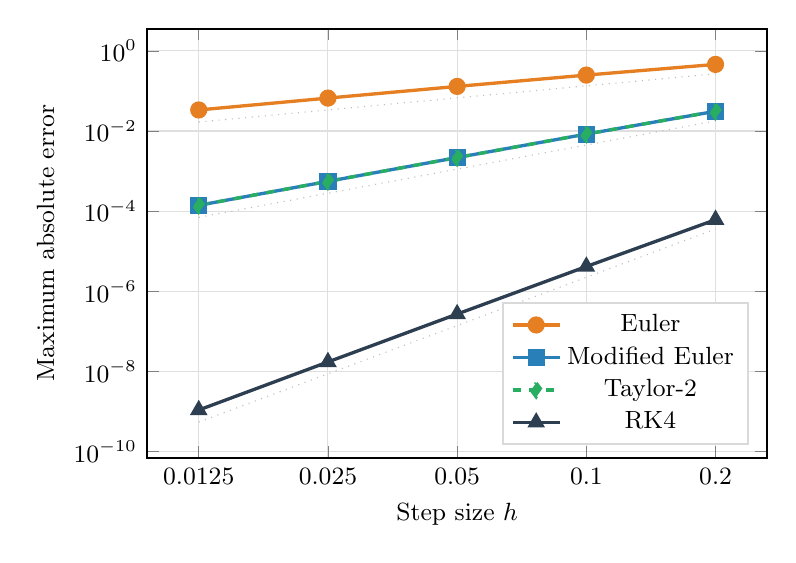
\begin{tikzpicture}\begin{axis}[width=0.78\textwidth,height=0.58\textwidth,xmode=log,ymode=log,xlabel={Step size $h$},ylabel={Maximum absolute error},grid=both,legend pos=south east,legend style={font=\small, fill=white, draw=gray!30},xtick={0.0125,0.025,0.05,0.1,0.2},xticklabels={0.0125,0.025,0.05,0.1,0.2},minor xtick={}]
\addplot[color=myorange,mark=*,mark options={fill=myorange}] coordinates {(0.2,4.5992e-01) (0.1,2.4908e-01) (0.05,1.2997e-01) (0.025,6.6436e-02) (0.0125,3.3594e-02)};\addlegendentry{Euler}
\addplot[color=myblue,mark=square*,mark options={fill=myblue}] coordinates {(0.2,3.1147e-02) (0.1,8.4020e-03) (0.05,2.1815e-03) (0.025,5.5577e-04) (0.0125,1.4025e-04)};\addlegendentry{Modified Euler}
\addplot[color=mygreen,mark=diamond*,dashed,mark options={fill=mygreen}] coordinates {(0.2,3.1147e-02) (0.1,8.4020e-03) (0.05,2.1815e-03) (0.025,5.5577e-04) (0.0125,1.4025e-04)};\addlegendentry{Taylor-2}
\addplot[color=myblack,mark=triangle*,mark options={fill=myblack}] coordinates {(0.2,6.1384e-05) (0.1,4.1686e-06) (0.05,2.7161e-07) (0.025,1.7332e-08) (0.0125,1.0946e-09)};\addlegendentry{RK4}
\addplot[gray!50,thin,dotted,forget plot] coordinates {(0.0125,1.6797e-02) (0.2,2.6875e-01)};
\addplot[gray!50,thin,dotted,forget plot] coordinates {(0.0125,7.0127e-05) (0.2,1.7953e-02)};
\addplot[gray!50,thin,dotted,forget plot] coordinates {(0.0125,5.4731e-10) (0.2,3.5868e-05)};
\end{axis}\end{tikzpicture}
\caption{Log--log plot of $E_{\max}$ against $h$ for Problem~1. Dotted lines show $O(h)$, $O(h^2)$ and $O(h^4)$ references. Modified Euler and Taylor-2 coincide exactly.}
\end{figure}
\begin{figure}[H]\centering
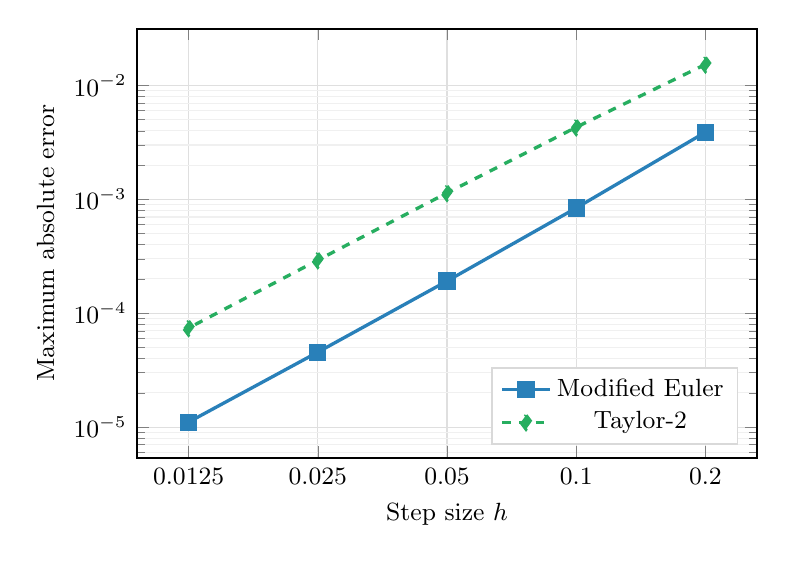
\begin{tikzpicture}\begin{axis}[width=0.78\textwidth,height=0.58\textwidth,xmode=log,ymode=log,xlabel={Step size $h$},ylabel={Maximum absolute error},grid=both,legend pos=south east,legend style={font=\small, fill=white, draw=gray!30},xtick={0.0125,0.025,0.05,0.1,0.2},xticklabels={0.0125,0.025,0.05,0.1,0.2},minor xtick={}]
\addplot[color=myblue,mark=square*,mark options={fill=myblue}] coordinates {(0.2,3.8850e-03) (0.1,8.3993e-04) (0.05,1.9159e-04) (0.025,4.5463e-05) (0.0125,1.1053e-05)};\addlegendentry{Modified Euler}
\addplot[color=mygreen,mark=diamond*,dashed,mark options={fill=mygreen}] coordinates {(0.2,1.5313e-02) (0.1,4.3007e-03) (0.05,1.1377e-03) (0.025,2.9244e-04) (0.0125,7.4120e-05)};\addlegendentry{Taylor-2}
\end{axis}\end{tikzpicture}
\caption{Problem~2: Modified Euler is more accurate than Taylor-2 at every step size, with the error ratio approaching the predicted value $7$.}
\end{figure}
\begin{figure}[H]\centering
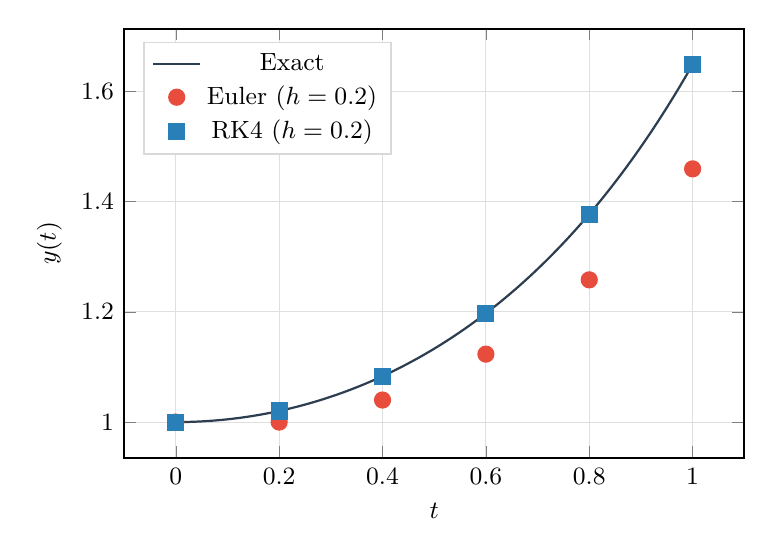
\begin{tikzpicture}\begin{axis}[width=0.78\textwidth,height=0.58\textwidth,xlabel={$t$},ylabel={$y(t)$},grid=both,legend pos=north west,legend style={font=\small, fill=white, draw=gray!30}]
\addplot[myblack,thick,domain=0:1,samples=80]{exp(x^2/2)};\addlegendentry{Exact}
\addplot[only marks,myred,mark=*,mark options={fill=myred}] coordinates {(0,1.00000) (0.2,1.00000) (0.4,1.04000) (0.6,1.12320) (0.8,1.25798) (1,1.45926)};\addlegendentry{Euler ($h=0.2$)}
\addplot[only marks,myblue,mark=square*,mark options={fill=myblue}] coordinates {(0,1.00000) (0.2,1.02020) (0.4,1.08329) (0.6,1.19722) (0.8,1.37713) (1,1.64872)};\addlegendentry{RK4 ($h=0.2$)}
\end{axis}\end{tikzpicture}
\caption{Exact solution, Euler and RK4 for Problem~2 at $h=0.2$.}
\end{figure}
\begin{figure}[H]\centering
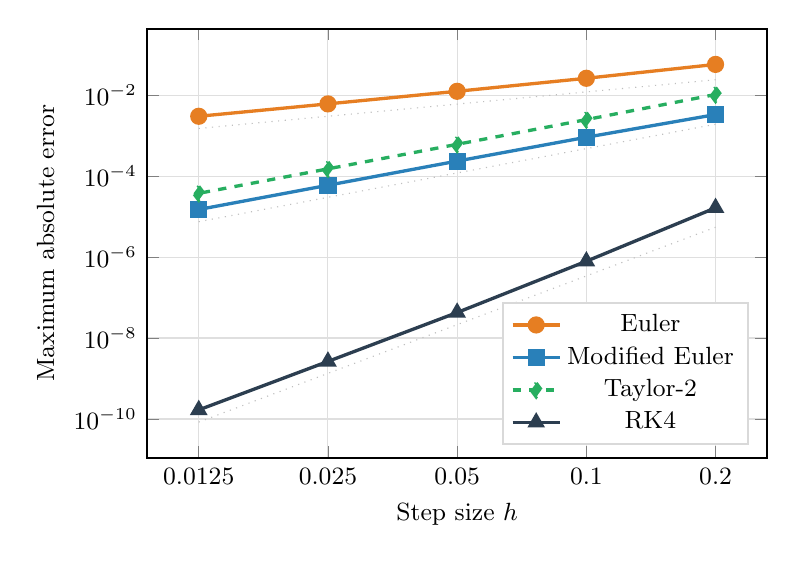
\begin{tikzpicture}\begin{axis}[width=0.78\textwidth,height=0.58\textwidth,xmode=log,ymode=log,xlabel={Step size $h$},ylabel={Maximum absolute error},grid=both,legend pos=south east,legend style={font=\small, fill=white, draw=gray!30},xtick={0.0125,0.025,0.05,0.1,0.2},xticklabels={0.0125,0.025,0.05,0.1,0.2},minor xtick={}]
\addplot[color=myorange,mark=*,mark options={fill=myorange}] coordinates {(0.2,5.7931e-02) (0.1,2.6320e-02) (0.05,1.2547e-02) (0.025,6.1264e-03) (0.0125,3.0271e-03)};\addlegendentry{Euler}
\addplot[color=myblue,mark=square*,mark options={fill=myblue}] coordinates {(0.2,3.3383e-03) (0.1,9.1858e-04) (0.05,2.3633e-04) (0.025,5.9761e-05) (0.0125,1.5017e-05)};\addlegendentry{Modified Euler}
\addplot[color=mygreen,mark=diamond*,dashed,mark options={fill=mygreen}] coordinates {(0.2,1.0448e-02) (0.1,2.5059e-03) (0.05,6.1394e-04) (0.025,1.5188e-04) (0.0125,3.7742e-05)};\addlegendentry{Taylor-2}
\addplot[color=myblack,mark=triangle*,mark options={fill=myblack}] coordinates {(0.2,1.6544e-05) (0.1,7.9098e-07) (0.05,4.2699e-08) (0.025,2.6414e-09) (0.0125,1.6741e-10)};\addlegendentry{RK4}
\addplot[gray!50,thin,dotted,forget plot] coordinates {(0.0125,1.5136e-03) (0.2,2.4217e-02)};
\addplot[gray!50,thin,dotted,forget plot] coordinates {(0.0125,7.5086e-06) (0.2,1.9222e-03)};
\addplot[gray!50,thin,dotted,forget plot] coordinates {(0.0125,8.3703e-11) (0.2,5.4856e-06)};
\end{axis}\end{tikzpicture}
\caption{Log--log plot of $E_{\max}$ against $h$ for the nonlinear Problem~7.}
\end{figure}

\subsection{Empirical order of convergence}
Table~4 gives the fitted orders. The pairwise orders from $h=0.1$ and $0.05$ differ from the fitted ones by at most $0.07$. The values lie close to the theoretical orders; small excesses (such as $4.14$ for RK4 on Problem~7 and $2.11$ for Heun on Problem~2) are pre-asymptotic effects.

\begin{table}[H]\centering
\caption{Empirical order of convergence (least-squares slope over $h=0.2,\dots,0.0125$).}
\begin{tabular}{@{}ccccc@{}}\toprule
Problem & Euler & Mod.\ Euler & Taylor-2 & RK4\\\midrule
1 & 0.95 & 1.95 & 1.95 & 3.95 \\
2 & 0.95 & 2.11 & 1.93 & 4.07 \\
3 & 0.96 & 1.97 & 1.95 & 3.98 \\
4 & 1.02 & 2.03 & 1.99 & 4.04 \\
5 & 1.02 & 2.02 & 2.02 & 4.03 \\
6 & 0.97 & 1.96 & 2.00 & 3.96 \\
7 & 1.06 & 1.95 & 2.03 & 4.14\\
\midrule
Theoretical & 1 & 2 & 2 & 4\\\bottomrule
\end{tabular}
\end{table}

\subsection{Computational cost}
To compare cost, we found by direct search the smallest number of steps $N$ for which each method reaches the RK4 error at $h=0.2$ on Problem~1 ($E_{\max}=6.14\times10^{-5}$). This is a count of function evaluations, not a runtime measurement.
\begin{center}
\begin{tabular}{@{}lccc@{}}\toprule
Method & Steps $N$ & $f$-evaluations & Extra\\\midrule
Euler & 44,283 & 44,283 & ---\\
Modified Euler & 122 & 244 & ---\\
Taylor-2 & 122 & 122 & 122 evaluations of $Df$\\
RK4 & 5 & 20 & ---\\\bottomrule
\end{tabular}
\end{center}
For this target and problem, RK4 needs about $2{,}200$ times fewer function evaluations than Euler and about $12$ times fewer than Modified Euler. The advantage will differ for other problems and tolerances; RK4's four evaluations per step also cost more than Euler's one when the target accuracy is loose.

\section{Conclusion}
Four explicit single-step methods were compared on seven non-stiff IVPs (five linear, two nonlinear). RK4 was the most accurate and, for the fixed-accuracy case examined, the cheapest. Empirical orders matched the theoretical orders $1,2,2,4$. Propagating the leading LTE coefficients through the variational equation gave asymptotic global-error constants that predicted the observed Heun-to-Taylor error ratios on all seven problems, including the two nonlinear ones. For constant-coefficient linear ODEs the two methods are identical; elsewhere, either can win depending on the equation.

\paragraph{Limitations.} The study uses seven problems, a single interval $[0,1]$, scalar equations and explicit methods only. The LTE-based predictions were verified numerically on these problems, not proved in general. Future work should treat stiff problems with implicit methods (BDF, Radau), systems of ODEs, and adaptive step-size control.

\section*{Acknowledgment}
The author thanks his supervisor, Department of Mathematics, Northwest University, Kano, for supervision, valuable comments, and for endorsing this work for arXiv submission.

\section*{Conflicts of interest}
The author declares no conflict of interest.

\section*{Data Availability}
All data and analyses are included in this article. MATLAB code and figures are available at \url{https://github.com/Sadiq-Dambatta/single-step-ODE-methods}.

\begin{thebibliography}{99}
\bibitem{kreyszig} Kreyszig, E. (2011). \emph{Advanced Engineering Mathematics}, 10th ed. Wiley, Hoboken, NJ.

\bibitem{hairer} Hairer, E., N{\o}rsett, S.~P., and Wanner, G. (1993). \emph{Solving Ordinary Differential Equations I: Nonstiff Problems}, 2nd ed. Springer, Berlin.

\bibitem{burden} Burden, R.~L., and Faires, J.~D. (2011). \emph{Numerical Analysis}, 9th ed. Brooks/Cole, Boston, MA.

\bibitem{sastry} Sastry, S.~S. (2012). \emph{Introductory Methods of Numerical Analysis}, 5th ed. PHI Learning, New Delhi.

\bibitem{lambert} Lambert, J.~D. (1991). \emph{Numerical Methods for Ordinary Differential Systems: The Initial Value Problem}. Wiley, Chichester.

\bibitem{stoer} Stoer, J., and Bulirsch, R. (2002). \emph{Introduction to Numerical Analysis}, 3rd ed. Springer, New York.

\bibitem{gerald} Gerald, C.~F., and Wheatley, P.~O. (2004). \emph{Applied Numerical Analysis}, 7th ed. Pearson, Boston, MA.

\bibitem{atkinson} Atkinson, K.~E. (1989). \emph{An Introduction to Numerical Analysis}, 2nd ed. Wiley, New York.

\bibitem{islam} Islam, M.~A. (2015). A comparative study on numerical solutions of initial value problems (IVP) for ordinary differential equations (ODE) with Euler and Runge--Kutta methods. \emph{American Journal of Computational and Applied Mathematics}, 5(3), 78--84.

\bibitem{workineh} Workineh, Y., Mekonnen, H., and Belew, B. (2024). Numerical methods for solving second-order initial value problems of ordinary differential equations with Euler and Runge--Kutta fourth-order methods. \emph{Frontiers in Applied Mathematics and Statistics}, 10, 1360628. doi:10.3389/fams.2024.1360628

\bibitem{salleh} Salleh, I., Ab Aziz, A., and Baki, N.~A. (2024). Comparison between Runge--Kutta method, Euler method and Modified Euler method for different order of ordinary differential equation. \emph{Journal of Advanced Mechanical Engineering Applications}, 5(2), 24--29.

\bibitem{audu} Audu, K.~J., et al. (2025). An investigative comparison of higher-order Runge--Kutta techniques for resolving first-order differential equations. \emph{Turkish Journal of Science and Technology}, 20(1), 141--158. doi:10.55525/tjst.1433935

\bibitem{butcher} Butcher, J.~C. (2016). \emph{Numerical Methods for Ordinary Differential Equations}, 3rd ed. Wiley, Chichester.

\bibitem{henrici} Henrici, P. (1962). \emph{Discrete Variable Methods in Ordinary Differential Equations}. Wiley, New York.
\end{thebibliography}
\end{document}